\section{An\'alisis de resultados}\label{sec:analisis}
Una vez que el algoritmo est\'a totalmente desarrollado y es funcional, se lanzan un compendio de ejecuciones con distintas combinaciones de par\'ametros con el objetivo de ver cu\'an bueno es.
En un intento de mejorar la comprensi\'on de todas las ejecuciones realizadas, se va a dividir esta secci\'on en dos ep\'igrafes. \\

En el primero de ellos se hace un an\'alisis de los resultados obtenidos haciendo variaciones en los par\'ametros del algoritmo gen\'etico. Estos son el n\'umero de \'arboles, el n\'umero de iteraciones y el tipo de periodo.\\

M\'as tarde, en el segundo ep\'igrafe, se van a comparar los resultados obtenidos, a trav\'es de los mejores par\'ametros, con otro algortimo de naturaleza parecida desarrollado en un art\'iculo.\\


\subsection{An\'alisis de par\'ametros}

Para medir el rendimiento del algoritmo en distintas situaciones, se han propuestos varios periodos de diferente longitud y que presentan distintas tendencias. Por sencillez, todos han sido seleccionados del mismo valor de bolsa, \textit{Banco Santander}.\\

Para obtener una mejor comprensi\'on, se han definido cinco configuraciones de par\'ametros. Cada configuraci\'on tiene sus par\'ametros establecidos en la figura \ref{fig:params}. Estas configuraciones, dependiendo de la longitud del periodo, pueden tardar desde unos minutos en ejecutar hasta cuatro horas en el caso m\'as grande.\\

     	\begin{figure}[H]
     		\centering\leftskip=52px
     		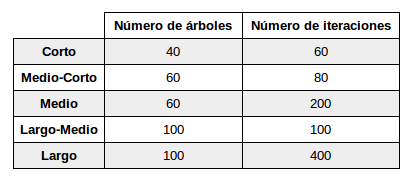
\includegraphics[scale=0.65]{imagenes/params.png}
     		\caption[Configuraciones de par\'ametros]{Configuraciones de par\'ametros.\\ Fuente: elaboraci\'on propia}
     		\label{fig:params}
     	\end{figure}

N\'otese que estas aproximaciones de tiempo ejecuci\'on se aportan a partir de la m\'aquina disponible, en este caso, de cuatro n\'ucleos y 3.4GHz.\\

En los casos expuestos a continuaci\'on se sigue siempre el mismo procedimiento. En primer lugar, el algoritmo gen\'etico efect\'ua, con los par\'ametros correspondientes, una serie de ejecuciones que terminan con una poblaci\'on evolucionada. De esta poblaci\'on obtenida, se selecciona el mejor de los individuos y se prueba tanto en el periodo de entrenamiento como en el periodo de prueba.\\

\subsubsection{Periodo largo}

En la primera de las ejecuciones, el periodo de entrenamiento comprende desde el 1 de abril de 2012 hasta el 1 de enero de 2016, por tanto, corresponde con un periodo bastante largo. De forma coherente, el periodo de prueba empieza el 1 de enero de 2016 y finaliza el 1 de mayo de 2019. Al comparar los perfiles de los precios en sendos periodos en las gr\'aficas, que se muestran a continuaci\'on, se puede observar que son parecidos, lo que deber\'ia mejorar los resultados.\\

     	\begin{figure}[H]
     		\centering\leftskip=-75px
     		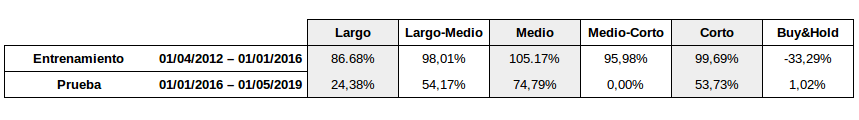
\includegraphics[scale=0.60]{imagenes/Large_period.png}
     		\caption[Ejecuci\'on en un periodo largo ascendente-descendente]{Ejecuci\'on en un periodo largo ascendente-descendente. Las cantidades mostradas son el porcentaje de beneficio respecto al presupuesto inicial.\\ Fuente: elaboraci\'on propia}
     		\label{fig:large_period}
     	\end{figure}
     	
A priori puede parecer que los resultados, que se pueden ver en la figura \ref{fig:large_period} son muy buenos. Pero, en realidad, muestran algunas carencias que se hacen obvias cuando se ve el calendario de inversi\'on.\\

Lo primero que destaca en la figura \ref{fig:large_period_mtrain}, que representa el calendario de inversi\'on del algoritmo con par\'ametros de perfil medio, es que la gran mayor\'ia de las ganancias proviene de una \'unica compraventa. El resto de inversiones son de poca duraci\'on y apenas si producen ganancias. La causa de este hecho puede ser una falta de especializaci\'on. A lo largo de la ejecuci\'on, alg\'un \'arbol ha conseguido hacer esa transacci\'on tan ventajosa y, a partir de esta, no se ha conseguido mejorar pr\'acticamente nada.\\

Es claro que, una inversi\'on de compra y venta algo m\'as r\'apida nos habr\'ia aportado una mayor ganacia.\\

Cuando analizamos el periodo de prueba, representado en la figura \ref{fig:large_period_mtest}, obtenemos un perfil similar. Se ha ajustado de manera muy eficiente una \'unica compraventa. Si bien es cierto que esa transacci\'on es casi perfecta, hay otras transacciones v\'alidas que no se han ejecutado.\\

     	\begin{figure}[H]
     		\centering\leftskip=30px
     		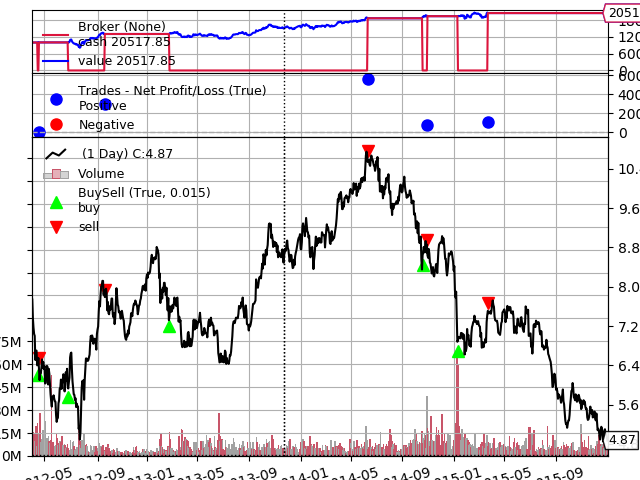
\includegraphics[scale=0.75]{imagenes/L_Medium_train.png}
     		\caption[Calendario de inversi\'on del periodo de entrenamiento largo.]{Calendario de inversi\'on del periodo de entrenamiento largo con par\'ametros de perfil Medio.\\ Fuente: elaboraci\'on propia}
     		\label{fig:large_period_mtrain}
     	\end{figure}
     	
     	\begin{figure}[H]
     		\centering\leftskip=30px
     		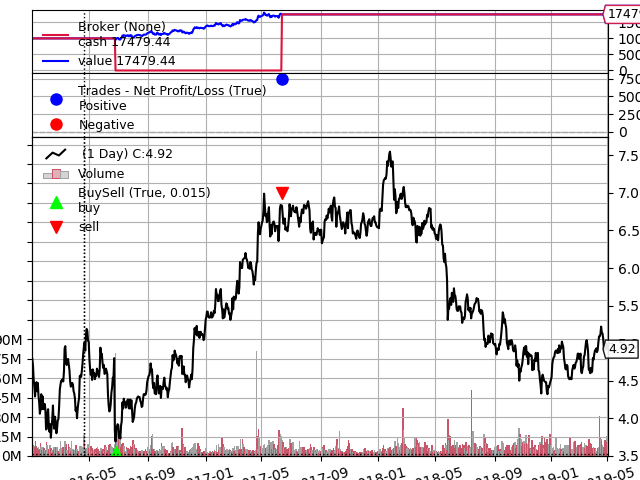
\includegraphics[scale=0.75]{imagenes/L_Medium_test.png}
     		\caption[Calendario de inversi\'on del periodo de prueba largo]{Calendario de inversi\'on del periodo de prueba largo con par\'ametros de perfil Medio.\\ Fuente: elaboraci\'on propia}
     		\label{fig:large_period_mtest}
     	\end{figure}     	

En resumen, los peridos largos dan muchas posibilidades de compraventa que nuestro algoritmo no sabe aprovechar. La parte positiva es que la mayor\'ia de las veces, cuando invierte, lo hace con beneficio. No obstante, en ocasiones, puede que no invierta y tengamos un modelo f\'util, como es el caso de la ejecuci\'on de par\'ametros de perfil Medio-Corto.\\

\subsubsection{Periodo medio}

En este segundo caso, se han elegido dos periodos distintos. En el primer periodo, claramente alcista, el entrenamiento comprende desde el 29 de septiembre de 2002 hasta el 29 de septiembre de 2003. Por otro lado, el periodo de prueba empieza el 29 de septiembre de 2003 y finaliza el mismo d\'ia de 2004. \\

El segundo periodo, de car\'acter bajista, est\'a formulado tambi\'en de a\~no en a\~no, el entrenamiento comienza el 1 de noviembre de 2009 y la prueba empieza el 1 de noviembre de 2010.\\

Una vez m\'as, se han tomado fechas en las que los perfiles de los precios se asemejan. \\

     	\begin{figure}[H]
     		\centering\leftskip=-75px
     		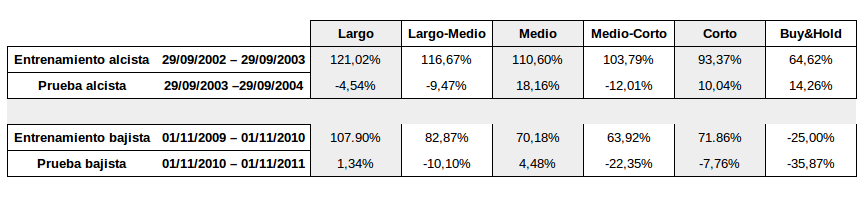
\includegraphics[scale=0.60]{imagenes/Medium_period.png}
     		\caption[Ejecuciones en un periodo medio alcista y en un periodo medio bajista]{Ejecuciones en un periodo medio alcista y en un periodo medio bajista. Las cantidades mostradas son el porcentaje de beneficio respecto al presupuesto inicial.\\ Fuente: elaboraci\'on propia}
     		\label{fig:medium_period}
     	\end{figure}
     	
En esta ocasi\'on, los resultados son significativamente peores. Con motivo de ilustrar la adaptaci\'on de los modelos obtenidos en el periodo de entrenamiento, se han tomado periodos de prueba ligeramente peores, es decir, el precio tiende, significativamente, a bajar m\'as que en el entrenamiento.\\

En todos los casos, el modelo obtenido con el algoritmo gen\'etico fue mejor que la estrategia \textit{Buy\&Hold} evaluados en el periodo de entrenamiento. Esto quiere decir que el algoritmo es capaz de encontrar condiciones de compra y venta que reportan beneficios en el periodo de aprendizaje. Sin embargo, estas condiciones no devuelven buenos resultados en periodos ligeramente distintos. De hecho, incluso en periodos alcistas, se pierde dinero cuando el modelo en el entrenamiento consigue sacar un 121.02\% de beneficios.\\

Otro punto que se puede destacar es la irregularidad del algoritmo. Habitualmente, otros algoritmos tienden a sobreaprender cuando se insiste demasiado en los datos de entrenamiento. As\'i pues, es habitual encontrar un punto de entrenamiento a partir del cual los resultados obtenidos en las pruebas empeoran.\\

En este algoritmo propuesto, los resultados obtenidos  para el periodo de prueba parecen variar de forma independiente al periodo anterior. Tras m\'ultiples ejecuciones con los mismos par\'ametros se puede observar como, en ocasiones, los resultados var\'ian de forma significativa. Este hecho puede ser la causa de una alta aleatoriedad en algoritmo debida a, posiblemente, la gran cantidad de mutaciones necesarias y la aleatoriedad de la primera generaci\'on.\\

     	\begin{figure}[H]
     		\centering\leftskip=40px
     		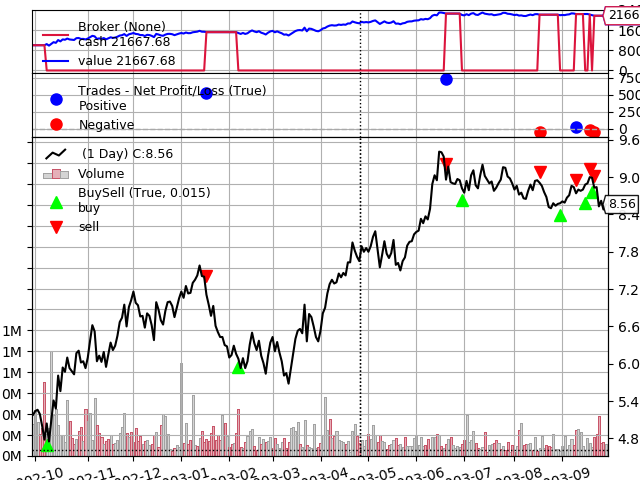
\includegraphics[scale=0.66]{imagenes/M_Large-Medium_train.png}
     		\caption[Calendario de inversi\'on del periodo de entrenamiento largo.]{Calendario de inversi\'on del periodo de entrenamiento alcista, longitud media y con par\'ametros de perfil Medio-Corto.\\ Fuente: elaboraci\'on propia}
     		\label{fig:medium_period_mtrain}
     	\end{figure}
     	
     	\begin{figure}[H]
     		\centering\leftskip=40px
     		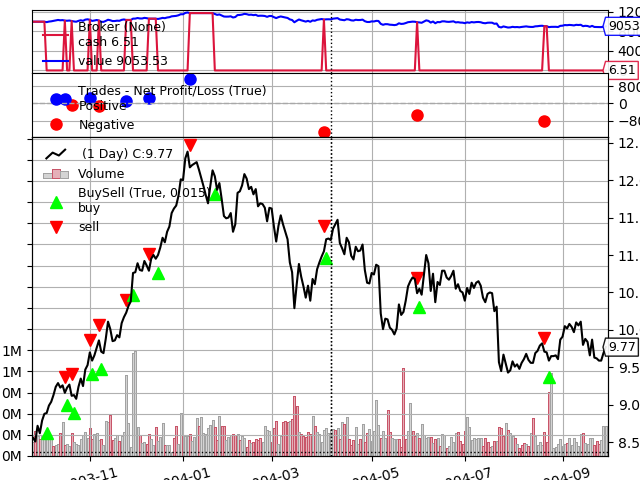
\includegraphics[scale=0.66]{imagenes/M_Large-Medium_test.png}
     		\caption[Calendario de inversi\'on del periodo de prueba medio]{Calendario de inversi\'on del periodo de prueba alcista, longitud media y con par\'ametros de perfil Medio-Corto.\\ Fuente: elaboraci\'on propia}
     		\label{fig:medium_period_mtest}
     	\end{figure} 

En las figuras \ref{fig:medium_period_mtrain} y \ref{fig:medium_period_mtest} puede observarse bastante bien esta baja adaptaci\'on. En el periodo de entrenamiento se hacen varias inversiones de unas semanas, e incluso de varios meses, entre las cuales se deja un margen de tiempo hasta que es un buen momento de compra. Por el contrario, en el periodo de prueba apenas si hay unas semanas en las que el modelo no tiene nada comprado, es decir, siempre que vende intenta comprar inmediatamente.\\

Se considera, como consecuencia de este hecho, la hip\'otesis de que el algoritmo tiene un buen aprendizaje pero una mala adaptaci\'on a otros periodos.\\

     	
\subsubsection{Periodo corto}

Para la \'ultima de las ejecuciones de par\'ametros, se han escogido tambi\'en dos periodos pero, esta vez, se ha tomado un periodo alcista y un periodo lateral. Este segundo es algo complicado, pues el periodo de entrenamiento es lateral pero el de prueba tiene tendencia bajista. \\

En primer lugar, el periodo alcista tiene su entrenamiento desde el 1 de julio de 2016 y hasta el 22 de octubre de 2016. Por otro lado, el periodo de prueba empieza a partir de entonces y hasta el 1 de febrero de 2017.\\

En segundo lugar, el periodo lateral comprende un poco m\'as de tres meses. El periodo de entrenamiento empieza el 1 de enero de 2018 y, por su parte, el periodo de prueba comienza el 22 de abril de 2018. La simulaci\'on termina, finalmente, el 22 de julio de 2018. Como ya se ha adelantado, no se esperan buenos resultados. Los modelos generados tienen poca capacidad de adaptaci\'on y, como hemos tomado periodos de entrenamiento y prueba con perfiles muy distintos, la adaptaci\'on debe ser bastante peor.\\

     	\begin{figure}[H]
     		\centering\leftskip=-75px
     		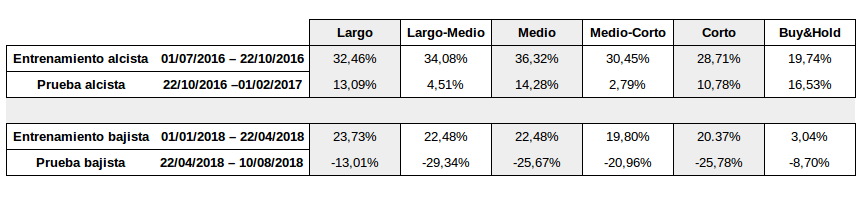
\includegraphics[scale=0.60]{imagenes/Short_period.png}
     		\caption[Ejecuciones en un periodo corto alcista y en un periodo corto lateral]{Ejecuciones en un periodo corto alcista y en un periodo corto lateral. Las cantidades mostradas son el porcentaje de beneficio respecto al presupuesto inicial.\\ Fuente: elaboraci\'on propia}
     		\label{fig:short_period}
     	\end{figure}

Como se observa en la figura \ref{fig:short_period}, en los periodos cortos no se obtienen buenos resultados. De hecho, en el caso del periodo lateral, y prueba bajista, los resultados son p\'esimos. Mientras que, en el entrenamiento, la estrategia propia supera con creces a la estrategia \textit{Buy\&Hold}, en la prueba tiene p\'erdidas estrepitosas al ser un periodo bajista. Esto confirma la hip\'otesis de la baja adaptaci\'on del algoritmo.\\

     	\begin{figure}[H]
     		\centering\leftskip=30px
     		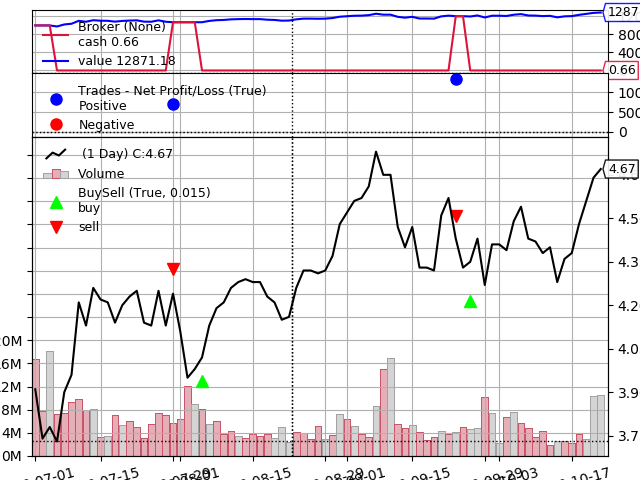
\includegraphics[scale=0.70]{imagenes/S_Short_train.png}
     		\caption[Calendario de inversi\'on del periodo de entrenamiento corto alcista.]{Calendario de inversi\'on del periodo de entrenamiento corto y alcista con perfil de par\'ametros Corto.\\ Fuente: elaboraci\'on propia}
     		\label{fig:short_period_uptrain}
     	\end{figure}
     	
En la figura \ref{fig:short_period_uptrain}, correspondiente al periodo alcista de entrenamiento, se encuentra un modelo generado con perfil de par\'ametros corto que invierte de una forma muy eficiente, esto es, compra en los m\'inimos y vende en los m\'aximos. \\

Teniendo esta regla como referencia, se analiza el mismo modelo ejecutado, esta vez, en el periodo de prueba en la figura \ref{fig:short_period_uptest}. Este periodo tiene un perfil de precio distinto, los m\'inimos y m\'aximos no son tan destacables. No obstante, el algoritmo ha generado un modelo que, tal y como se intuye, est\'a intentando hacer algo similar a lo realizado en el periodo del que aprendi\'o. Las primeras transacciones son torpes y demasiado abundantes, produciendo p\'erdidas con las comisiones.	Por tanto, a pesar de ser un periodo alcista, no tiene tanto \'exito como la estrategia de \textit{Buy\&Hold}.\\
     	
     	\begin{figure}[H]
     		\centering\leftskip=30px
     		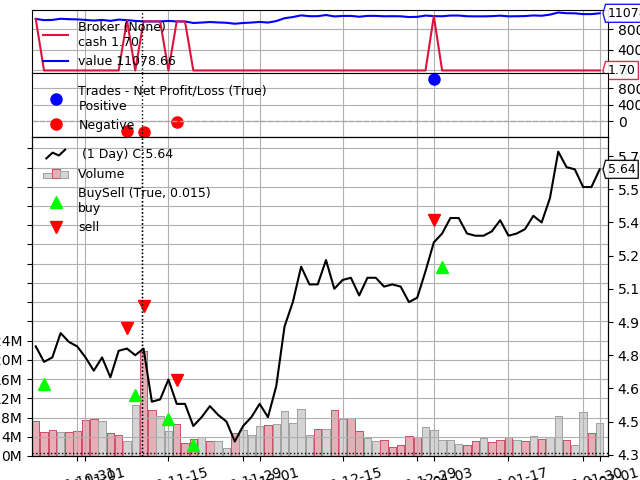
\includegraphics[scale=0.70]{imagenes/S_Short_test.png}
     		\caption[Calendario de inversi\'on del periodo de prueba corto alcista]{Calendario de inversi\'on del periodo de prueba corto y alcista con perfil de par\'ametros Corto.\\ Fuente: elaboraci\'on propia.}
     		\label{fig:short_period_uptest}
     	\end{figure} 
     	
Por \'ultimo, se propone hacer una an\'alisis del periodo entrenado con perfil lateral pero probado con un perfil bajista. Las figuras \ref{fig:short_period_downtrain} y \ref{fig:short_period_downtest} contiene los calendarios de inversi\'on de estas simulaciones realizadas con configuraci\'on de par\'ametros Largo.\\

En el entrenamiento se tiene una inversi\'on muy ajustada, pr\'acticamente inmejorable. No obstante, esto podr\'ia ser fruto de un sobreaprendizaje. Por su parte, en el periodo de prueba, se observan los mismos patrones de compra y venta. Pero al ser las oscilaciones del precio m\'as peque\~nas que en el caso anterior, las comisiones se llevan esos escasos beneficios que pudiera tener.\\

En contraposici\'on, encontramos un punto a favor, la precisi\'on para encontrar los m\'inimos. Los indicadores parecen ser unas buenas herramientas para detectar estos. N\'otese que, tras una acentuada ca\'ida durante el primer mes, se compra en el \'ultimo momento antes de la subida. Por tanto, aunque los resultados no son para nada correctos, las se\~nales de compra y venta no son demasiado err\'oneas. \\
     	
      	\begin{figure}[H]
      		\centering\leftskip=40px
      		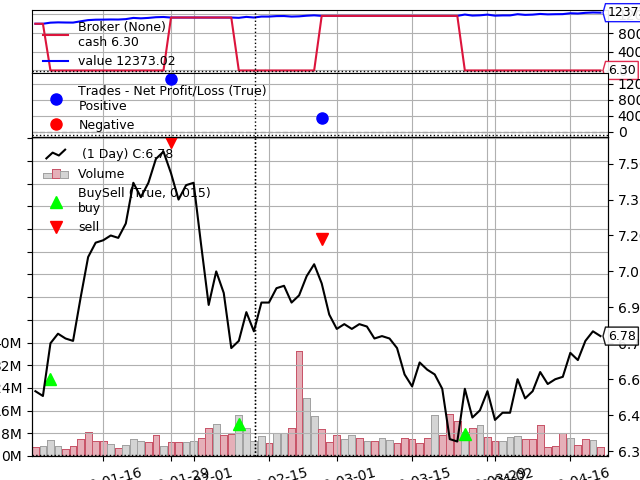
\includegraphics[scale=0.66]{imagenes/S_Large_train.png}
      		\caption[Calendario de inversi\'on del periodo de entrenamiento corto lateral]{Calendario de inversi\'on del periodo de entrenamiento corto lateral con perfil de par\'ametros Largo.\\ Fuente: elaboraci\'on propia.}
      		\label{fig:short_period_downtrain}
      	\end{figure}
      	
     	\begin{figure}[H]
     		\centering\leftskip=40px
     		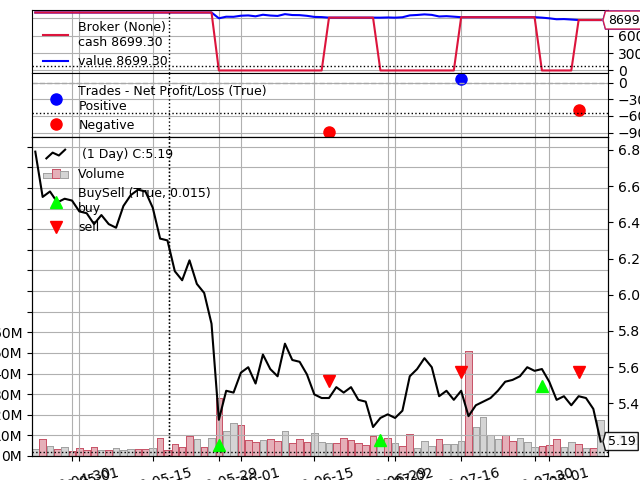
\includegraphics[scale=0.66]{imagenes/S_Large_test.png}
     		\caption[Calendario de inversi\'on del periodo de prueba corto bajista]{Calendario de inversi\'on del periodo de prueba corto bajista con perfil de par\'ametros Largo.\\ Fuente: elaboraci\'on propia.}
     		\label{fig:short_period_downtest}
     	\end{figure} 

\subsection{Contraste con otras estrategias}


\newpage

\section{Conclusiones}
Para finalizar este proyecto, se va a hacer una s\'intesis en la que repasaremos los objetivos que propusimos al inicio.\\

En primer lugar, se prentend\'ia realizar un algoritmo evolutivo basado en \'arboles para extraer informaci\'on de se\~nales de compra y venta. El dise\~no de este algoritmo se especifica en el punto \ref{sec:algorithm}. El c\'odigo que corresponde al dise\~no no se puede incluir en la memoria por motivos de espacio, no obstante, se incluye como anexo.\\

En el segundo punto se propuso implementar mejoras de tiempo para hacer el algoritmo eficiente. Tras las mejoras realizadas en la secci\'on \ref{sec:timeimprove}, el software mostr\'o una reducci\'on de tiempo considerable. En el caso de la ejecuci\'on m\'as larga, entrenamiento de cuatro a\~nos y prueba de tres con poblaci\'on de 100 \'arboles y 400 iteraciones, el tiempo total fue de algo menos de cuatro horas. La ejecuci\'on m\'as corta, por su parte, de tres meses de entrenamiento y otros tres de prueba con 40 \'arboles y 60 iteraciones, tuvo un tiempo de apenas dos minutos. Recordando que las ejecuciones fueron realizadas en un ordenador convencional de cuatro n\'ucleos y 3.4GHz, la eficiencia es satisfactoria.\\

En el tercer punto se marc\'o como objetivo analizar los resultados obtenidos en diferentes situaciones y, asimismo, comparar estos con otros resultados de la bibliograf\'ia. Gracias al desarrollo de la secci\'on \ref{sec:analisis} podemos considerar este objetivo cumplido.\\

Por \'ultimo, se incluy\'o un punto adicional en el que se ped\'ia mejorar los resultados obtenidos en la literatura.\\

(.)\\

(.)\\

(.)\\


\subsection{Perfil del algoritmo}



\subsection{Trabajos futuros}


